\documentclass[12pt,a4paper]{article}
\usepackage[utf8]{inputenc}
\usepackage[T1]{fontenc}
\usepackage[spanish,es-tabla]{babel}
\usepackage{lmodern}
\usepackage[margin=2.5cm]{geometry}
\usepackage{graphicx}
\usepackage{float}
\usepackage{booktabs}
\usepackage{tabularx}
\usepackage{array}
\usepackage{enumitem}
\usepackage{xcolor}
\usepackage{tikz}
\usetikzlibrary{positioning,arrows.meta,calc}
\usepackage{hyperref}
\usepackage{setspace}
\usepackage{fancyhdr}
\setlength{\headheight}{15pt}
\usepackage{pdflscape}
\graphicspath{{../diagramas/}}
\hypersetup{colorlinks=true,linkcolor=blue!50!black,urlcolor=blue!50!black}
\makeatletter\g@addto@macro\UrlBreaks{\do\-}\makeatother
\setstretch{1.1}
\setlength{\parindent}{0pt}
\setlength{\parskip}{6pt}
\newcommand{\pendiente}[1]{\textcolor{red}{\textbf{[POR COMPLETAR: #1]}}}
\pagestyle{fancy}\fancyhf{}
\lhead{Banco de Preguntas Saber}
\rhead{Documento de arquitectura -- Segunda iteración}
\cfoot{\thepage}
\begin{document}
\begin{titlepage}
\centering
{\Large Universidad del Cauca\\Facultad de Ingeniería Electrónica y Telecomunicaciones\\Programa de Ingeniería de Sistemas\par}
\vspace{2cm}
{\huge\bfseries Banco de Preguntas Saber\par}
\vspace{0.5cm}
{\Large Documento de Arquitectura -- Iteración 2\par}
\vspace{1cm}
{Equipo ``Sin Nombre''\par}
\vspace{0.4cm}
Juan Manuel Meneses Daza\\Juan Sebastian Muñoz Ruiz\\Juan Sebastian Molano Bolaños\\Santiago Rodríguez Bolaños
\vfill
Ingeniería de Software II -- 2026.2\\Popayán, noviembre de 2026
\end{titlepage}
\tableofcontents\newpage

\section{Resumen}
Este documento describe lo verificado en el repositorio del Banco de Preguntas Saber Pro. La iteración separa autenticación, banco de preguntas, revisión por pares y auditoría en servicios independientes. La interfaz de escritorio conserva operaciones locales del primer corte; por ello la migración no es completa. La escalabilidad operativa no se ha medido ni demostrado. La base principal de esta descripción es el código de los cuatro servicios, \texttt{docs/decisiones-iteracion-2.md} y \texttt{docs\_2/SAD.pdf}.

\section{Requisitos funcionales}
Las historias y criterios se expresan en lenguaje de negocio. El alcance de HU01--HU04 procede de \texttt{docs/decisiones-iteracion-2.md}; la parte de HU05 se limita a la revisión implementada.

\subsection{Épica: administrar usuarios (HU01)}
Como persona usuaria, quiero registrarme e iniciar sesión para acceder a las funciones que corresponden a mi rol. El sistema debe evitar logins repetidos, proteger las contraseñas y no permitir el acceso con credenciales incorrectas o con una cuenta inactiva.

\subsection{Épica: gestionar preguntas (HU02)}
Como autor, quiero crear, consultar, filtrar y corregir preguntas para construir un banco útil para la preparación Saber Pro. Solo se edita el contenido cuando está en borrador. Una pregunta contiene contexto, pregunta, opciones, respuesta correcta y datos académicos necesarios.

\subsection{Épica: asegurar calidad de preguntas (HU03)}
Como autor, quiero recibir una explicación cuando una pregunta no cumple las reglas acordadas para corregirla antes de que se incorpore al banco. Los criterios verificables se resumen en `RULES.md` y se aplican antes de guardar.

\subsection{Épica: administrar el ciclo de vida (HU04)}
Como autor, revisor o administrador, quiero que cada pregunta avance solo por etapas permitidas y que el historial muestre quién realizó cada cambio. Las preguntas archivadas no se reactivan ni se borran físicamente.

\subsection{HU05 implementada parcialmente: revisión por pares}
Como revisor, quiero tomar una revisión y registrar un dictamen para que el Banco avance la pregunta. El servicio impide que la revise su propio autor y exige observaciones al rechazar. La asignación automática y una rúbrica completa quedan fuera del alcance verificado.

\subsection{Roles y permisos observados}
\begin{tabularx}{\textwidth}{p{3.5cm}X}
\toprule Operación & Permiso verificado \\
\midrule
Crear o editar pregunta & \texttt{ADMINISTRADOR} o \texttt{AUTOR\_PREGUNTAS} \\
Cambiar estado & \texttt{ADMINISTRADOR}, \texttt{AUTOR\_PREGUNTAS} o \texttt{REVISOR} \\
Consultar preguntas y estadísticas & Se valida token; el controlador no aplica un rol específico \\
Tomar revisión o emitir dictamen & `REVISOR` o `ADMINISTRADOR`, con reglas de pertenencia \\
\bottomrule
\end{tabularx}

\section{Prototipos y usabilidad}
No hay prototipos de la iteración 2 verificables en los archivos fuente enumerados. \pendiente{El equipo debe adjuntar prototipos vigentes y resultados de evaluación de usabilidad.}

\section{Escenarios de calidad}
Los escenarios técnicos del SAD y MiniQAW se reexpresan como esfuerzo de las personas involucradas, no como rendimiento medido. Todas las cifras siguientes son \textbf{propuesta, por validar con el equipo y el profesor}; no son resultados obtenidos.
\begin{tabularx}{\textwidth}{p{3cm}X p{3cm}}
\toprule Atributo & Escenario de negocio & Medida propuesta \\
\midrule
Modificabilidad & Agregar o ajustar una regla de calidad de pregunta y revisar que no se afecten las demás reglas. & 4 personas-hora para cambio y pruebas; propuesta, por validar. \\
Seguridad & Revisar roles, token y respuestas ante intentos de acceso indebido. & 6 personas-hora para revisión manual y casos de prueba; propuesta, por validar. \\
Usabilidad & Una persona nueva crea y busca preguntas con instrucciones mínimas. & 30 minutos de persona usuaria para completar la primera tarea; propuesta, por validar. \\
Escalabilidad & Preparar una demostración de mayor carga y registrar el resultado. & 8 personas-hora para preparar y ejecutar una prueba inicial; propuesta, por validar. No se fija umbral de usuarios porque el código no tiene medición ni infraestructura escalable verificada. \\
Trazabilidad & Revisar si una pregunta que cambia de estado queda registrada en auditoría y revisión. & 4 personas-hora para prueba y análisis de fallos; propuesta, por validar. \\
\bottomrule
\end{tabularx}

\section{Modelo de datos}
Las tablas se verifican en las clases de configuración de Auth, Banco, Revisión y Auditoría. Los catálogos de roles y estados se almacenan como texto, no como tablas independientes. Las referencias de pregunta desde revisión/auditoría no son llaves foráneas entre bases.
\begin{figure}[p]\centering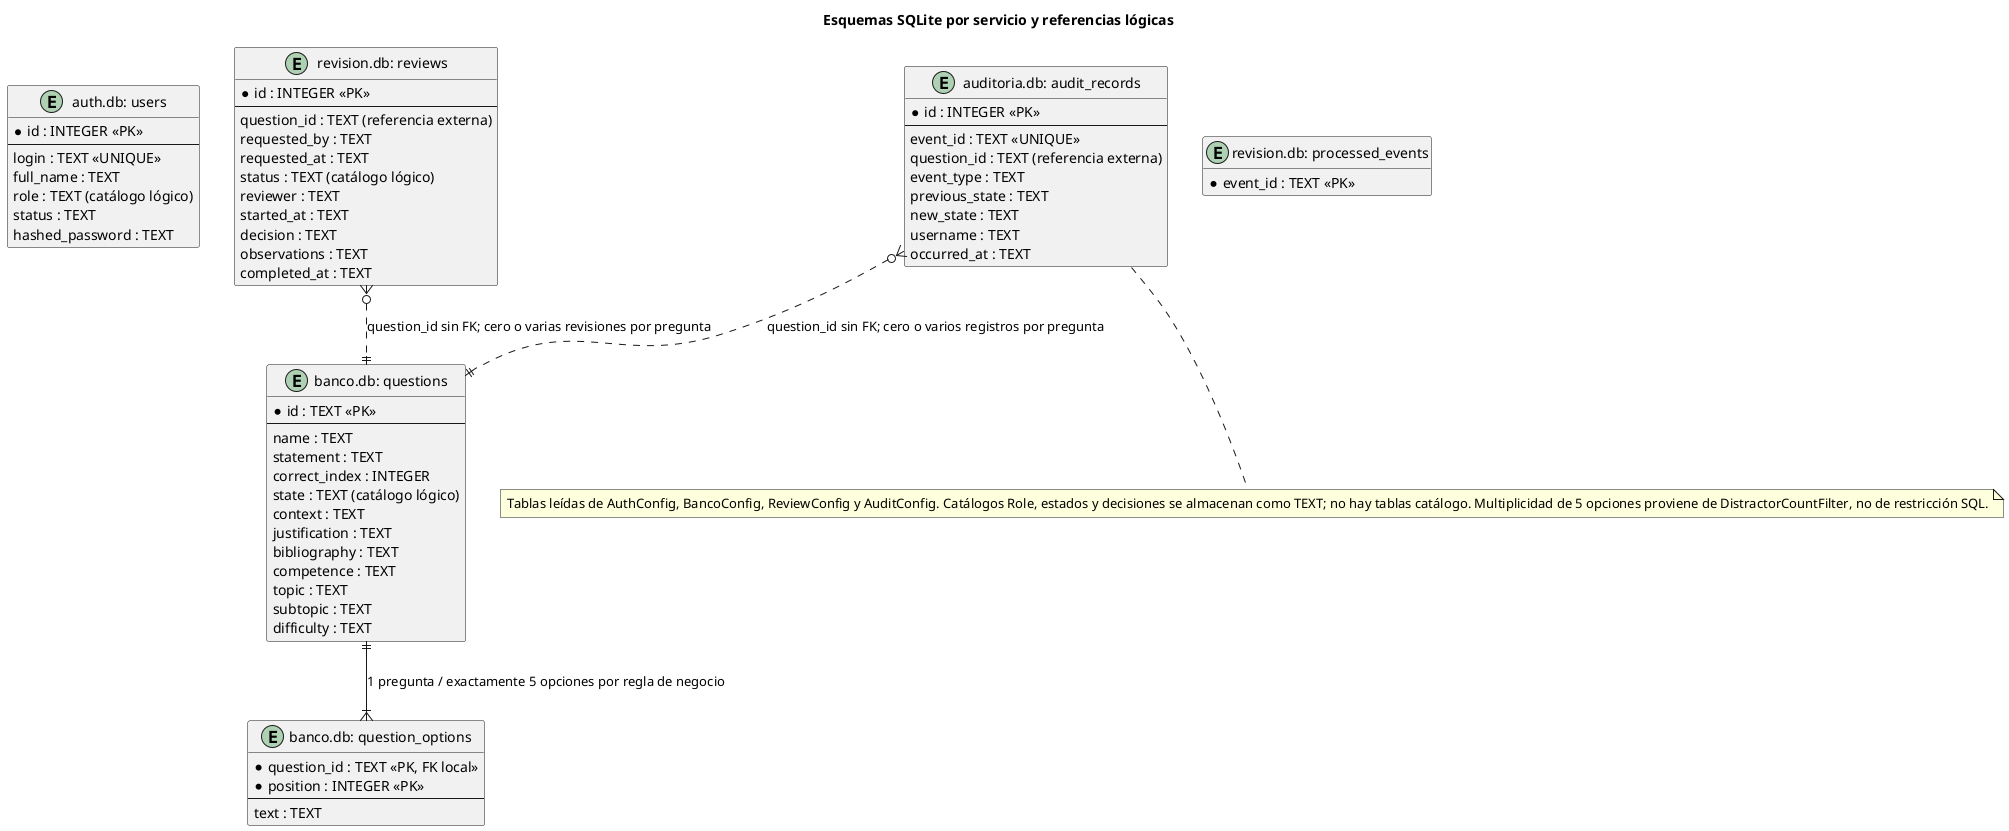
\includegraphics[width=0.78\textwidth]{06-er-bases.png}\caption{Esquemas por base de datos.}\end{figure}

\section{Arquitectura}
\subsection{Vista de contexto}
\begin{figure}[p]\centering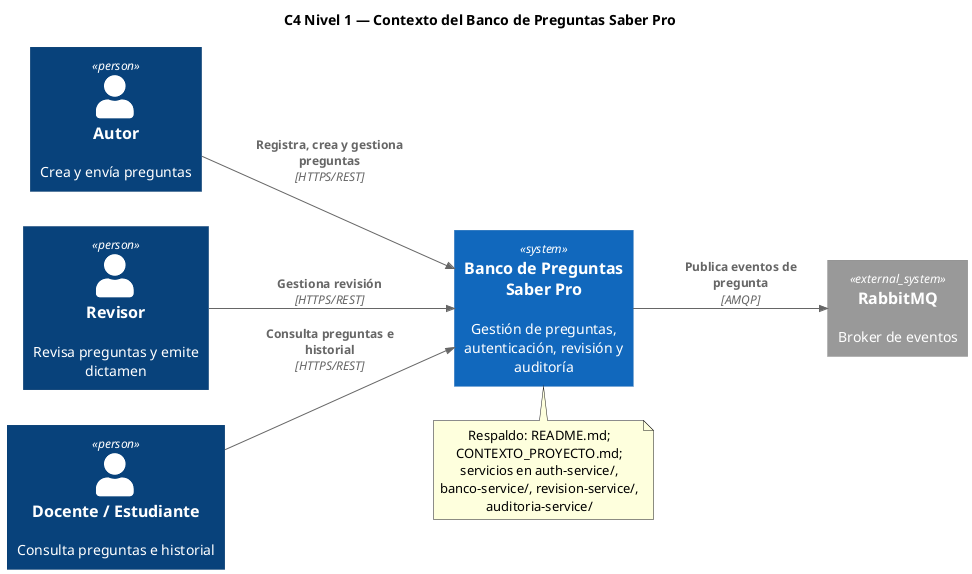
\includegraphics[width=0.78\textwidth]{01-contexto-c4.png}\caption{C4 nivel 1.}\end{figure}
\subsection{Vista de contenedores}
\begin{landscape}\begin{figure}[H]\centering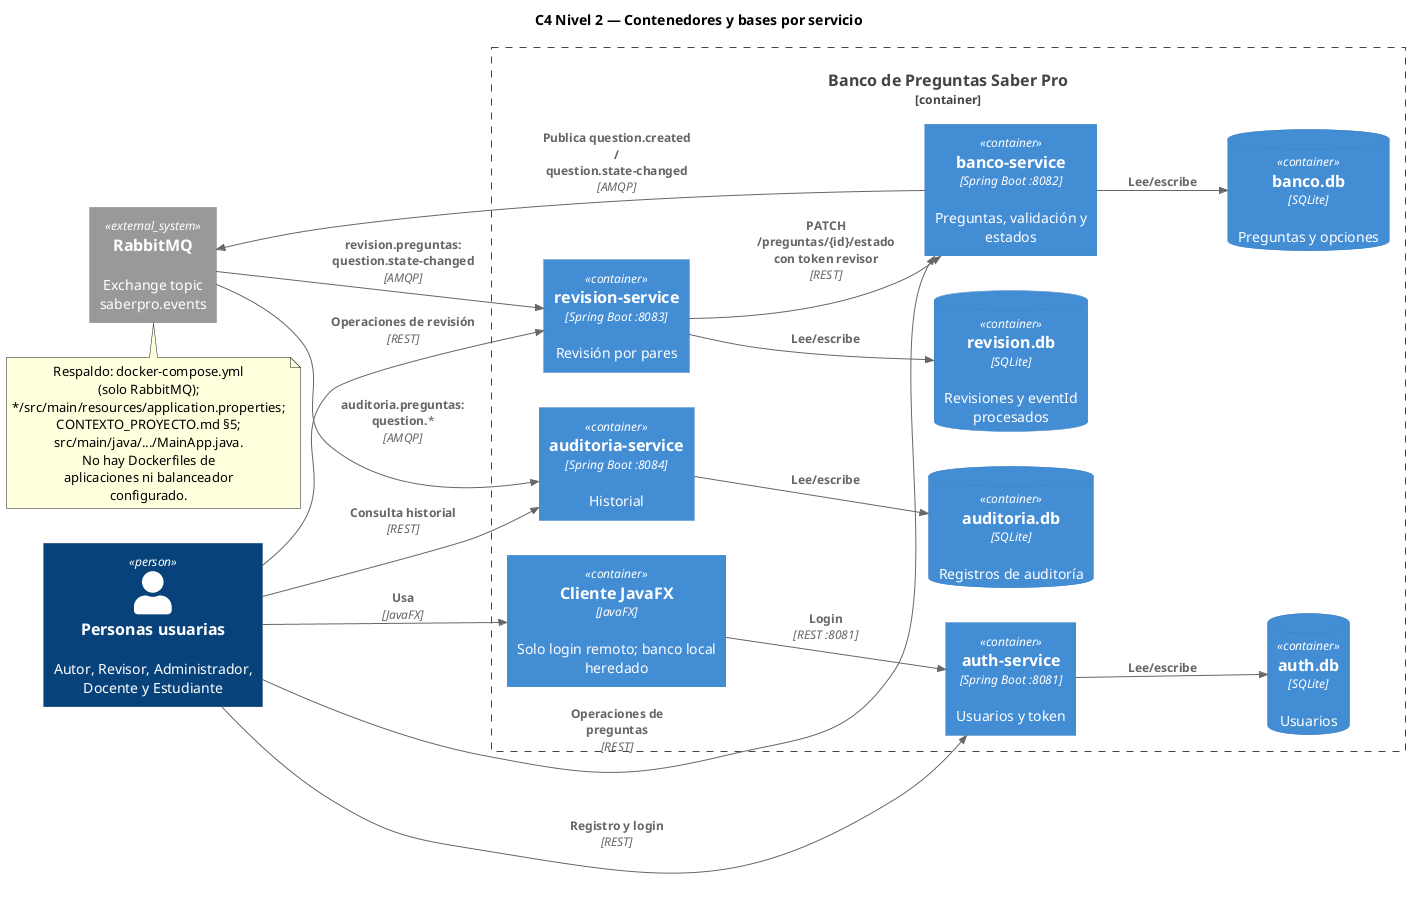
\includegraphics[width=0.94\linewidth]{02-contenedores-c4.png}\caption{C4 nivel 2: cuatro servicios, broker, bases y cliente.}\end{figure}\end{landscape}
\subsection{Vista de componentes}
\clearpage
\begin{landscape}\begin{figure}[p]\centering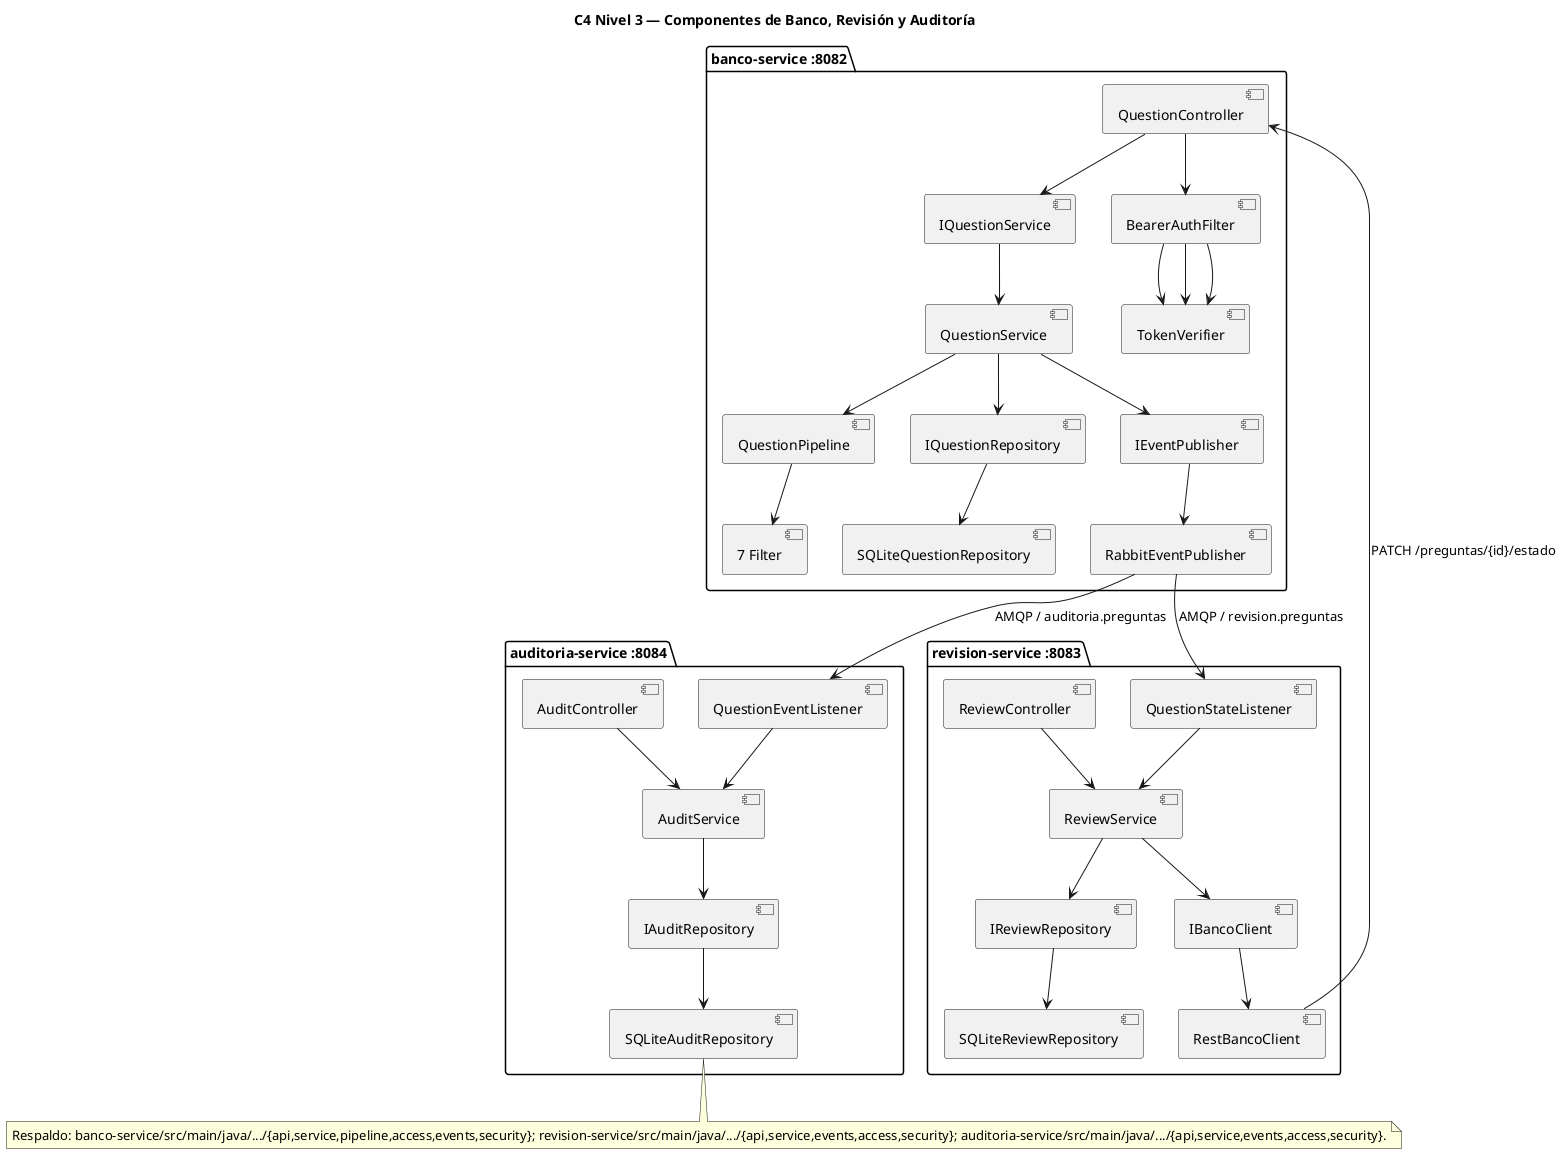
\includegraphics[width=0.82\linewidth]{03-componentes-c4.png}\caption{C4 nivel 3: Banco, Revisión y Auditoría.}\end{figure}\end{landscape}
\subsection{Vistas 4+1}
\begin{itemize}[leftmargin=*]
\item Lógica: dominios de preguntas, usuario, revisión y auditoría; véanse diagramas UML.
\item Desarrollo: cuatro módulos Maven y cliente JavaFX heredado.
\item Procesos: REST para operaciones y RabbitMQ para eventos; los consumidores registran identificadores procesados.
\item Física: configuración local con SQLite por servicio; `docker-compose.yml` define solo el broker.
\item Escenarios: crear pregunta y revisión por pares, descritos más adelante.
\end{itemize}
\subsection{Comunicación y eventos}
Auth emite tokens; Banco, Revisión y Auditoría los verifican localmente. Banco publica `question.created` y `question.state-changed` en `saberpro.events`; Auditoría consume ambos por `auditoria.preguntas`, Revisión consume cambios de estado por `revision.preguntas`. Revisión llama al Banco con el token del revisor. La publicación no tiene Outbox y los reintentos de consumidores no sustituyen a una DLQ.
\begin{figure}[p]\centering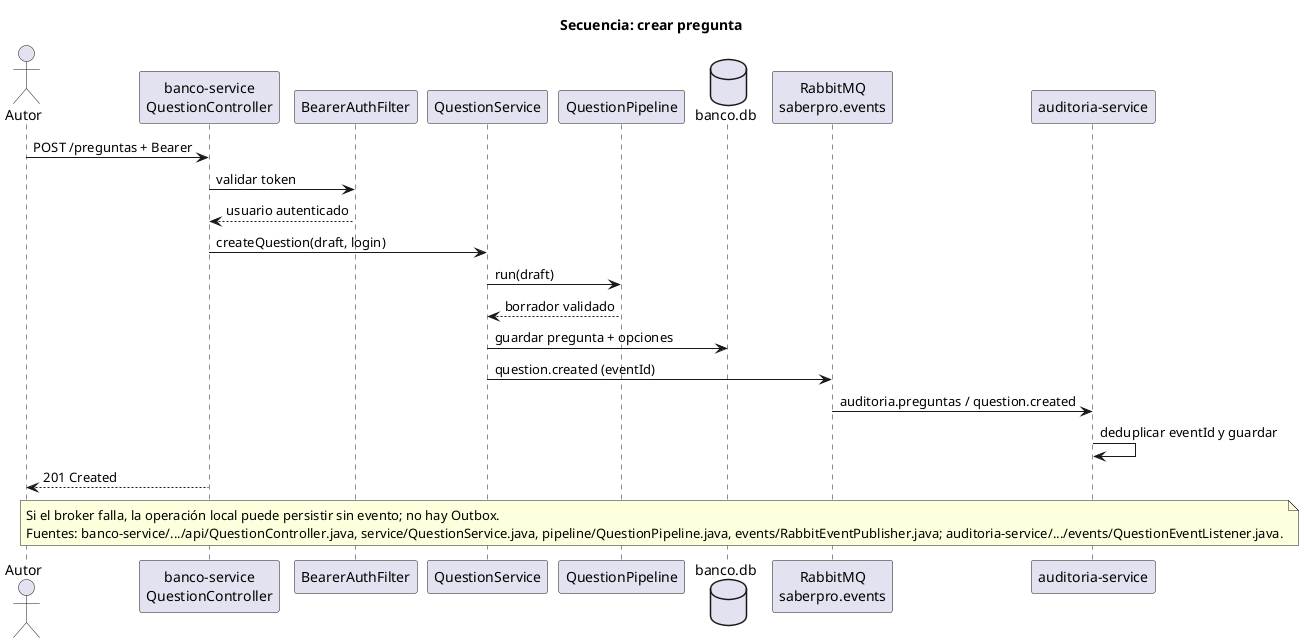
\includegraphics[width=0.78\textwidth]{07-secuencia-crear-pregunta.png}\caption{Secuencia de creación.}\end{figure}
\begin{figure}[p]\centering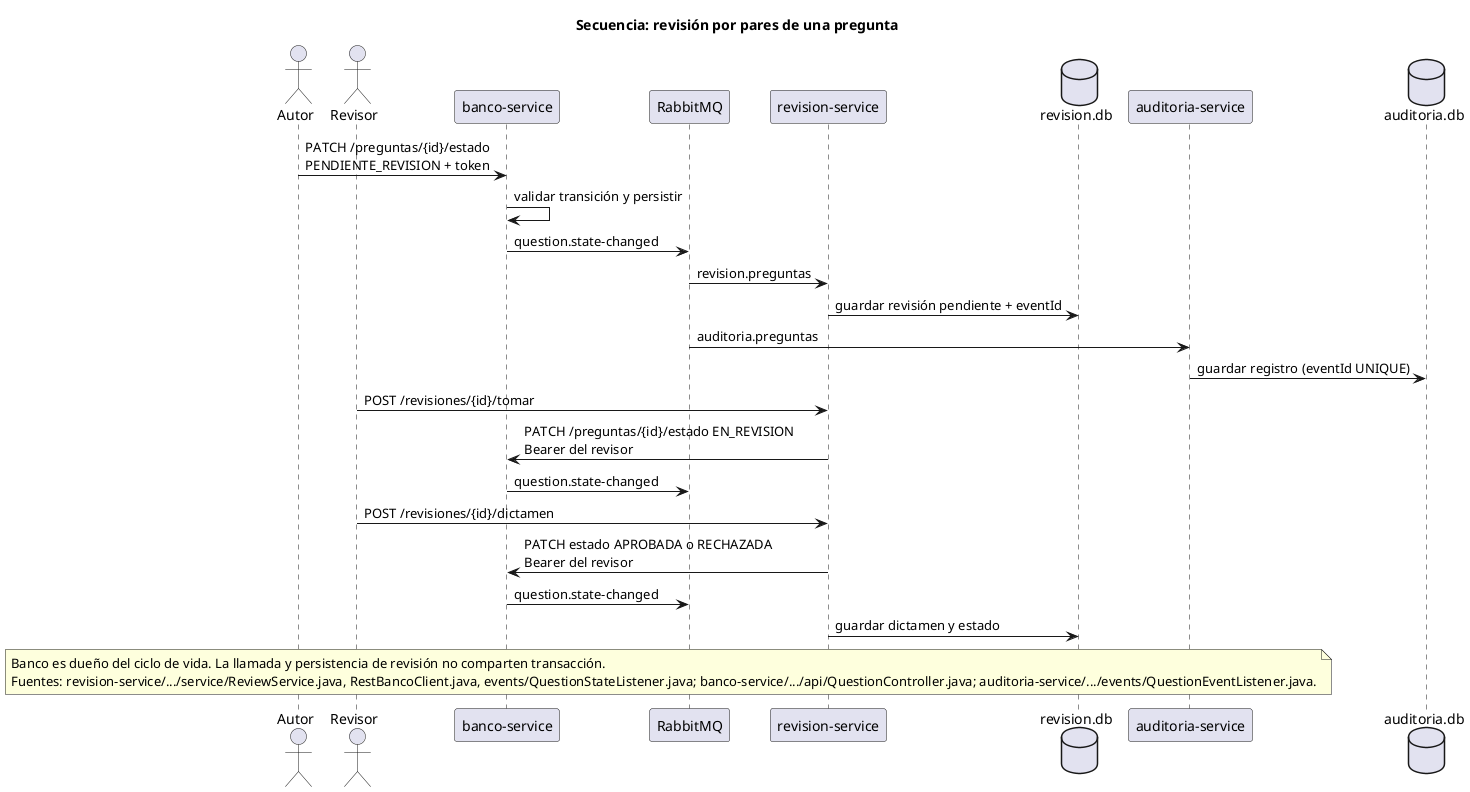
\includegraphics[width=0.78\textwidth]{08-secuencia-revision-pares.png}\caption{Secuencia de revisión por pares.}\end{figure}
\begin{figure}[p]\centering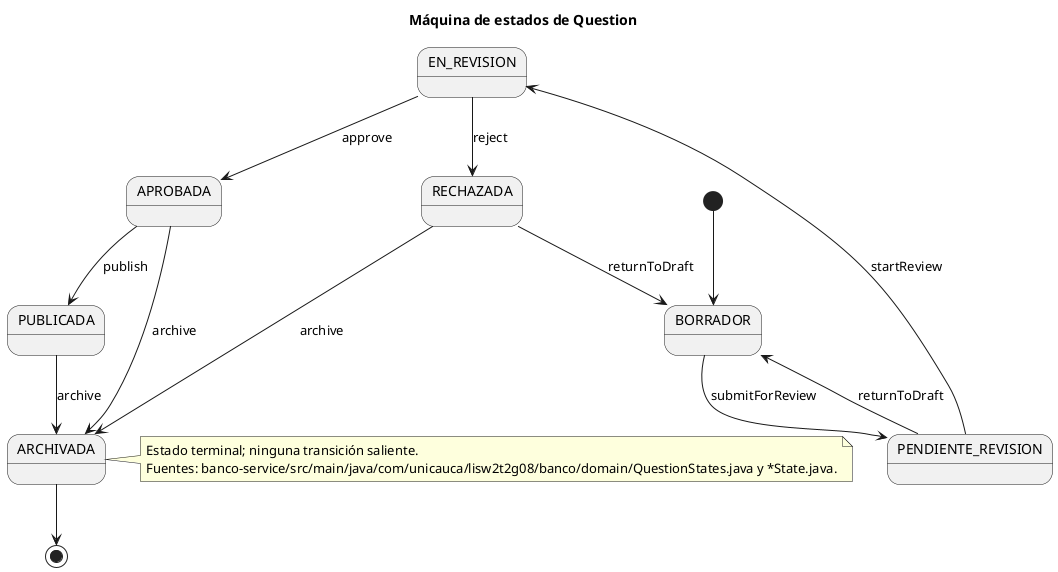
\includegraphics[width=0.78\textwidth]{09-estados.png}\caption{Estados de pregunta.}\end{figure}

\section{Información repetida entre servicios}
Se repiten roles, formato de token, códigos de estado y contratos de eventos. Se conservan copias locales para que los servicios no dependan de clases de otro módulo. Los cambios requieren compatibilidad y pruebas coordinadas; las referencias \texttt{question\_id} entre bases no son llaves foráneas. Ver \texttt{docs/REDUNDANCIAS.md}.

\section{Decisiones finales y patrones aplicados}
Decisiones finales: microservicios con eventos; una SQLite por servicio; token HMAC-SHA256 compartido; validación embebida; \texttt{revision-service} en lugar del servicio anterior de validación; jerarquía State; Pipeline de filtros; consumidores idempotentes por \texttt{eventId}. Los ADR individuales están en \texttt{docs/adr/}. Observer permanece en el cliente local de \texttt{src/}; no es el mecanismo de eventos entre servicios. La lista académica de patrones «vistos» requiere validación del profesor.

\section{Cumplimiento del Sprint 2}
La matriz detallada de evidencia y acciones está en \texttt{docs/CUMPLIMIENTO\_SPRINT2.md}. Conclusión: cumplimiento parcial; escalabilidad no demostrada.

\section{Pruebas}
\begin{itemize}
\item \texttt{auth-service}: 21; pasó.
\item \texttt{banco-service}: 94; pasó.
\item \texttt{revision-service}: 40; pasó.
\item \texttt{auditoria-service}: 9; pasó.
\item Monolito raíz: 158; pasó.
\end{itemize}
Ejecutadas con Maven el 2026-11-22. Los conteos no equivalen a cobertura; no se encontró medición de cobertura.

\section{Gestión del proyecto}
\pendiente{Jira: adjuntar Product Backlog, Sprint Backlog, Task Board y Burndown Chart como evidencia del curso.}

\section{Sustentación y repositorio}
Repositorio: \url{https://github.com/BastianRu/proyecto-saberpro-ing-software-II}.\\
\pendiente{Equipo: adjuntar enlace o evidencia del video de sustentación.}

\end{document}
